% Options for packages loaded elsewhere
\PassOptionsToPackage{unicode}{hyperref}
\PassOptionsToPackage{hyphens}{url}
%
\documentclass[
]{article}
\usepackage{lmodern}
\usepackage{amssymb,amsmath}
\usepackage{ifxetex,ifluatex}
\ifnum 0\ifxetex 1\fi\ifluatex 1\fi=0 % if pdftex
  \usepackage[T1]{fontenc}
  \usepackage[utf8]{inputenc}
  \usepackage{textcomp} % provide euro and other symbols
\else % if luatex or xetex
  \usepackage{unicode-math}
  \defaultfontfeatures{Scale=MatchLowercase}
  \defaultfontfeatures[\rmfamily]{Ligatures=TeX,Scale=1}
\fi
% Use upquote if available, for straight quotes in verbatim environments
\IfFileExists{upquote.sty}{\usepackage{upquote}}{}
\IfFileExists{microtype.sty}{% use microtype if available
  \usepackage[]{microtype}
  \UseMicrotypeSet[protrusion]{basicmath} % disable protrusion for tt fonts
}{}
\makeatletter
\@ifundefined{KOMAClassName}{% if non-KOMA class
  \IfFileExists{parskip.sty}{%
    \usepackage{parskip}
  }{% else
    \setlength{\parindent}{0pt}
    \setlength{\parskip}{6pt plus 2pt minus 1pt}}
}{% if KOMA class
  \KOMAoptions{parskip=half}}
\makeatother
\usepackage{xcolor}
\IfFileExists{xurl.sty}{\usepackage{xurl}}{} % add URL line breaks if available
\IfFileExists{bookmark.sty}{\usepackage{bookmark}}{\usepackage{hyperref}}
\hypersetup{
  pdftitle={LiterateRmd},
  pdfauthor={Kevin Lanning},
  hidelinks,
  pdfcreator={LaTeX via pandoc}}
\urlstyle{same} % disable monospaced font for URLs
\usepackage[margin=1in]{geometry}
\usepackage{graphicx}
\makeatletter
\def\maxwidth{\ifdim\Gin@nat@width>\linewidth\linewidth\else\Gin@nat@width\fi}
\def\maxheight{\ifdim\Gin@nat@height>\textheight\textheight\else\Gin@nat@height\fi}
\makeatother
% Scale images if necessary, so that they will not overflow the page
% margins by default, and it is still possible to overwrite the defaults
% using explicit options in \includegraphics[width, height, ...]{}
\setkeys{Gin}{width=\maxwidth,height=\maxheight,keepaspectratio}
% Set default figure placement to htbp
\makeatletter
\def\fps@figure{htbp}
\makeatother
\setlength{\emergencystretch}{3em} % prevent overfull lines
\providecommand{\tightlist}{%
  \setlength{\itemsep}{0pt}\setlength{\parskip}{0pt}}
\setcounter{secnumdepth}{-\maxdimen} % remove section numbering
\ifluatex
  \usepackage{selnolig}  % disable illegal ligatures
\fi

\title{LiterateRmd}
\author{Kevin Lanning}
\date{2021-02-07}

\begin{document}
\maketitle

\hypertarget{part-part-iii-towards-data-proficiency}{%
\section*{(PART) Part III Towards data
proficiency}\label{part-part-iii-towards-data-proficiency}}
\addcontentsline{toc}{section}{(PART) Part III Towards data proficiency}

\begin{center}\rule{0.5\linewidth}{0.5pt}\end{center}

In this part of the class we will get into the nuts and bolts of R.

\hypertarget{literate-programming-with-r-markdown}{%
\section{literate programming with R
markdown}\label{literate-programming-with-r-markdown}}

Showing your work, to (future) you as well as others, is a key part of
reproducible science. R Markdown documents facilitate this, as they
allow you to include comments, code, and results in a single place. But
before we consider R markdown, we begin with two more elemental ideas:
\emph{scripts} (R4DS, Chapter 6) and \emph{projects} (Chapter 8).

\hypertarget{scripts-are-files-of-code}{%
\subsection{scripts are files of code}\label{scripts-are-files-of-code}}

We begin with R4DS Chapter 6, which shows the R studio interface and
encourages you to save your work using scripts, written in the source
(editor) window in the upper left quadrant of the default R studio
screen.

Note the recommendations - for example, include packages (libraries) at
the beginning of your code. One more thing - in setting up R studio,
consider adjusting the ``insert spaces for tab'' setting to something
more than 2. This will allow you to more easily see the nested structure
of functions, loops, etc. - and will create a modest disincentive
against making these nested structures too deep or complex:

\begin{figure}
\centering
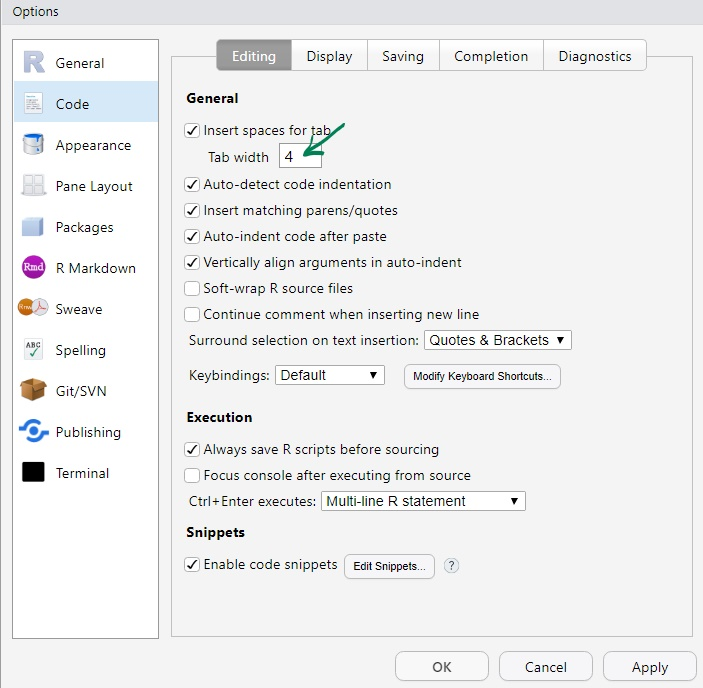
\includegraphics{images/RStudioOptions.jpg}
\caption{Fig 11.1: I use 4 spaces here. YMMV.}
\end{figure}

Note, too, the
\href{https://support.rstudio.com/hc/en-us/articles/205753617-Code-Diagnostics}{code
diagnostics} in R. Consider enabling all of these, including the R style
diagnostics, to help you keep your code readable:

\begin{figure}
\centering
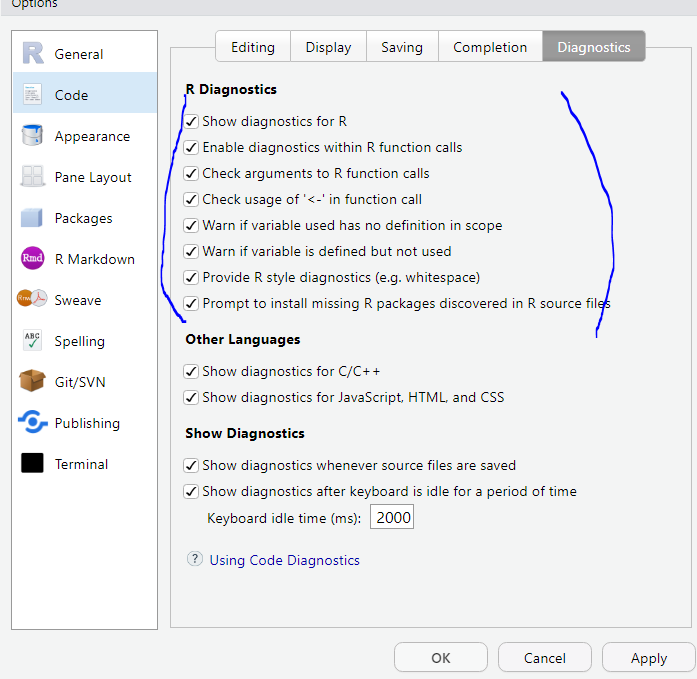
\includegraphics{images/codediagnostics.PNG}
\caption{Fig 11.2: Enable code diagnostics}
\end{figure}

\hypertarget{some-elements-of-coding-style}{%
\subsubsection{some elements of coding
style}\label{some-elements-of-coding-style}}

Good coding is often a combination of several skills ranging from
puzzle-solving to communication. I can't claim that these are \emph{the}
elements of coding style (apologies to Strunk \& White), but rather that
these are merely some of the elements.

Good coding is \textbf{clear} and thus commented. You are writing for
your future self as well as others, so be explicit about the purpose of
each chunk of code.

Good coding is \textbf{concise}. When you can write code in 3 lines
instead of 30, your code may be more clear and efficient. Take pleasure
in writing parsimonious, efficient code. But where efficiency and
clarity conflict, choose the latter.

Good code should be \textbf{complete}, including all steps from reading
the data to producing output. Where appropriate, comment-out (rather
than delete) informative errors, again for the future you.

Good code may be \textbf{creative}. The coolest solutions are those
which pull from and synthesize a number of ideas. Creativity often
requires walking away from a problem in order to ultimately arrive at a
solution (Wertheimer's \emph{Productive Thinking}).

Finally, good code should be \textbf{considered}. Reflect on the impacts
of your work - just because you can analyze something doesn't mean that
you should.

\hypertarget{projects-are-directories-containing-related-scripts}{%
\subsection{projects are directories containing related
scripts}\label{projects-are-directories-containing-related-scripts}}

You will save your work in \emph{projects} - which isolate your data and
scripts into different directories. (See r4ds, Chapter 8). To reinforce
the idea that your unit of analysis in R is ``the project'' rather than
``the script'', consider associating your Rmd filetype (see next
section) with your markdown editor, and only your Rproj filetype with R
studio.

Soon, it is likely that you will soon be working on R for different
things in parallel - for this and another class, for this class and your
thesis, or perhaps for two distinct types of analysis within your
thesis. When you open up an R project, you'll be in the right directory,
with the relevant files (and only the relevant files) at your fingertips
in the files pane.

\hypertarget{r-markdown-documents-integrate-rationale-script-and-results}{%
\subsection{R markdown documents integrate rationale, script, and
results}\label{r-markdown-documents-integrate-rationale-script-and-results}}

R Markdown documents allow you to include comments, scripts, and results
in a single place. The basics of R markdown are presented in Chapter 27
of R4DS. I encourage you to use R markdown for nearly everything you do
in R.

Within R studio, open up a new R markdown document. There are as many as
four parts of an R markdown document:

\begin{itemize}
\tightlist
\item
  A YAML (yet another markdown language) header
\item
  Text formatted in markdown
\item
  R code (chunks) surrounded by code fences
\item
  and, occasionally, inline code
\end{itemize}

There is a handy
\href{https://www.rstudio.com/wp-content/uploads/2015/02/rmarkdown-cheatsheet.pdf}{R
Markdown cheat sheet} which can give you a sense of what R markdown is
about. It describes eight steps, from ``workflow'' to ``publish'' (and a
ninth, ``learn more''). Don't worry about all of the detail here, but do
get a sense of how it works.

\begin{quote}
Exercise 11.1:

Working in groups, do the exercises in section 27.4.7 of R4DS.

Begin with the R markdown file that is included at the beginning of
Chapter 27. You can download it
\href{https://raw.githubusercontent.com/hadley/r4ds/master/rmarkdown/diamond-sizes.Rmd}{here}.

Study the code, and annotate it so that you have a better sense of how
it works. For example, ``this block loads needed libraries, then takes
the \_\_\_\_\_dataset and \_\_\_\_\_\_\_\_\_\_\_ .''

Play with the graph. Change one or more parameters of it to make it more
useful. Again, annotate your changes.
\end{quote}

\hypertarget{what-to-do-when-you-are-stuck}{%
\subsection{What to do when you are
stuck}\label{what-to-do-when-you-are-stuck}}

\begin{itemize}
\item
  Google. pay attention to your error messages
\item
  Ask for help, make your questions clear and reproducible (see R4DS
  Chapter 1)
\item
  Take a break, think outside the box and
  \href{https://www.google.com/search?newwindow=1\&safe=active\&rlz=1C1SQJL_enUS782US782\&q=Dictionary\#dobs=kludge}{kludge}
  something together if you have to
\item
  Document your struggle and your cleverness for a future you
\end{itemize}

\end{document}
